\documentclass[11pt]{article}
\usepackage[utf8]{inputenc}
\usepackage[dvips]{graphicx}
\usepackage{fancybox}
\usepackage{verbatim}
\usepackage{array}
\usepackage{latexsym}
\usepackage{alltt}
\usepackage{hyperref}
\usepackage{textcomp}
\usepackage{color}
\usepackage{amsmath}
\usepackage{amsfonts}
\usepackage{tabularx}
\usepackage{tikz}
\usepackage{fitch}  % to use fitch
\usepackage{float}
\usepackage{pgfplots}
\usepackage[hmargin=3cm,vmargin=5.0cm]{geometry}
%\topmargin=0cm
\topmargin=-2cm
\addtolength{\textheight}{6.5cm}
\addtolength{\textwidth}{2.0cm}
%\setlength{\leftmargin}{-5cm}
\setlength{\oddsidemargin}{0.0cm}
\setlength{\evensidemargin}{0.0cm}


\begin{document}

\section*{Student Information } 
%Write your full name and id number between the colon and newline
%Put one empty space character after colon and before newline
Full Name :  Anıl Eren Göçer \\
Id Number :  2448397 \\

\section*{Answer 1} 
\section*{a)}
For X and Y to be independent, they must satisfy the condition: \\ \\
\indent $f_{(X,Y)}(x,y) = f_X(x) . f_Y(y)$  \indent for all x \in [-1,1] , y \in [-1,1] \indent $(\star)$ \\ \\
where $f_X$ and $f_Y$ are marginal densities of X and Y respectively.  \\ \\
Now, let's calculate marginal densities, namely $f_X$ and $f_Y$. \\ \\

for x \in [-1,1]; \\

\int_{-\sqrt{1-x^2}}^{\sqrt{1-x^2}} f_{(X,Y)}(x,y)dy = \int_{-\sqrt{1-x^2}}^{\sqrt{1-x^2}}\dfrac{1}{\pi}dy = \dfrac{2\sqrt{1-x^2}}{\pi} \\ \\

for y \in [-1,1]; \\

\int_{-\sqrt{1-y^2}}^{\sqrt{1-y^2}} f_{(X,Y)}(x,y)dx = \int_{-\sqrt{1-y^2}}^{\sqrt{1-y^2}}\dfrac{1}{\pi}dx = \dfrac{2\sqrt{1-y^2}}{\pi} \\ \\

\noindent Observe that for $x^2 + y^2 \leq 1$  \\

$f_{(X,Y)}(x,y) = \dfrac{1}{\pi} \neq \dfrac{4\sqrt{1-x^2}\sqrt{1-y^2}}{\pi^2} = f_X(x).f_Y(y)$  \\ \\

\noindent So, they do not satisfy the condition $(\star)$. \\ \\

\noindent Hence, X and Y are \textbf{NOT} independent. 

\newpage

\section*{b)}
Marginal pdfs for X and Y denoted by $f_X(x)$ and $f_Y(y)$ respectively can be found as follows: \\

$f_X(x) = \int_{-\sqrt{1-x^2}}^{\sqrt{1-x^2}} f_{(X,Y)}(x,y)dy = \int_{-\sqrt{1-x^2}}^{\sqrt{1-x^2}}\dfrac{1}{\pi}dy = \dfrac{1}{\pi}y \big|_{-\sqrt{1-x^2}}^{\sqrt{1-x^2}}
=\dfrac{2\sqrt{1-x^2}}{\pi}$ \\ \\

$f_Y(y) = \int_{-\sqrt{1-y^2}}^{\sqrt{1-y^2}} f_{(X,Y)}(x,y)dx = \int_{-\sqrt{1-y^2}}^{\sqrt{1-y^2}}\dfrac{1}{\pi}dx = \dfrac{1}{\pi}x \big|_{-\sqrt{1-y^2}}^{\sqrt{1-y^2}}
=\dfrac{2\sqrt{1-y^2}}{\pi}$ \\ \\

\noindent Therefore ; \\

\textbf{marginal pdf of X is $f_X(x) = \dfrac{2\sqrt{1-x^2}}{\pi}$ \space , \indent x \in [-1,1]}
\\ \\

\textbf{marginal pdf of Y is \textbf{$f_Y(y) = \dfrac{2\sqrt{1-y^2}}{\pi}$} \space , \indent y $\in [-1,1]}$ 


\section*{c)}
$\mu_X = E(X) = \int_{-1}^{1} x f_X(x)dx = \int_{-1}^{1} \dfrac{x . 2 \sqrt{1-x^2}}{\pi} = \int_{-1}^{1} \dfrac{2x \sqrt{1-x^2}}{\pi}$ \\
 
\noindent \normalfont{applying the substitution:} \\

\noindent $u$ = $\sqrt{1-x^2}$\\
$du = -2xdx$ \\ 

\noindent \normalfont{the integral becomes:} \\

\noindent \int \dfrac{-\sqrt{u}}{\pi}du = \dfrac{-2}{3}\dfrac{u^{3/2}}{\pi} = \dfrac{-2}{3}\dfrac{(1-x^2)^{3/2}}{\pi} \\

\noindent \normalfont{putting boundaries;} \\ \\
$\dfrac{-2}{3} \dfrac{(1-x^2)^{3/2}}{\pi}\big|_{-1}^{1}$  = 0 \\\\

\noindent \textbf{Hence, expected value of X, E(X), is \textbf{0}.}\newpage

\section*{d)}
$\sigma^2 = Var(X) = \int_{-1}^{1}x^2f_X(x)dx - \mu^2 = \int_{-1}^{1}x^2f_X(x)dx -0^2 = \int_{-1}^{1}x^2f_X(x)dx = \int_{-1}^{1}\dfrac{x^2.2\sqrt{1-x^2}}{\pi} dx \\ =\dfrac{2}{\pi} \int_{-1}^{1}  x^2\sqrt{1-x^2} dx$ \\ \\

\noindent Now, let's compute the integral $\int x^2\sqrt{1-x^2}dx$, then put boundaries and then multiply it with  \dfrac{2}{\pi}.  \\ \\

\noindent Apply the substitution on $\int x^2\sqrt{1-x^2}dx$\space:  \\ 

\noindent $x = sin(u)$ \\
$dx = cos(u)du$ \\ \\

\noindent \int sin^2(u).\sqrt{1-sin^2(u)}.cos(u).du = \int sin^2(u).cos(u).cos(u).du = \int sin^2(u).cos^2(u).du = \dfrac{1}{4}\int sin^2(2u)du \newline = \dfrac{1}{4}\int \dfrac{1}{2}(1-cos(4u))du = \dfrac{1}{8}\int (1-cos(4u))du = 
\dfrac{1}{8}(u-\dfrac{sin(4u)}{4}) = \dfrac{1}{8}u - \dfrac{1}{32}sin(4u) \\ \\

\noindent Now back-substitute: \\ \\
\int x^2\sqrt{1-x^2}dx = \dfrac{1}{8}.arcsin(x) - \dfrac{1}{32}.sin(4.arcsin(x)) + C \\ \\

\noindent By putting boundaries; \\ \\

\noindent \int_{-1}^{1}x^2\sqrt{1-x^2}dx = [\dfrac{1}{8}arcsin(x)-\dfrac{1}{32}sin(4.arcsin(x)) + C] \big|_{-1}^{1} = \dfrac{\pi}{16} + \dfrac{\pi}{16} = \dfrac{\pi}{8} \\ \\

\noindent Multiply by \dfrac{2}{\pi}: \\ \\
Var(X) = \dfrac{2}{\pi} \int_{-1}^{1}x^2\sqrt{1-x^2} = \dfrac{2}{\pi} .\dfrac{\pi}{8} = \dfrac{1}{4} = 0.25 \\ \\ \\

\noindent Hence, variance of X, $Var(X)$ is \textbf{\dfrac{1}{4} = 0.25}. 




\newpage
\section*{Answer 2}


\section*{a)}
$T_A$ and $T_B$ are uniformly distributed on [0,100], so their marginal density functions are as follows: \\

$f_A(t_A)$ = $\dfrac{1}{100 - 0} = \dfrac{1}{100}$ \\
\indent f$_B(t_B)$ = $\dfrac{1}{100 - 0} = \dfrac{1}{100}$ \\ \\ \\

\noindent Because they are independent, their joint density function can be found as follows: \\ \\
\indent $f(t_A,t_B)$ = $f_A(t_A) . f_B(t_B)$ = $\dfrac{1}{100} . \dfrac{1}{100} = \dfrac{1}{10000}$ \\ \\

\noindent Their joint cumulative distribution function (cdf) can be found as follows: \\

$F(t_A,t_B) = \int \int f(t_A,t_B) . dt_A.dt_B$ = $\int \int \dfrac{1}{10000} .dt_A . dt_B$ = $\dfrac{t_A . t_B}{10000}$ \\

$F(t_A,t_B) $ =  $\dfrac{t_A . t_B}{10000} $



\section*{b)}





\tikzset{every picture/.style={line width=0.75pt}} %set default line width to 0.75pt        

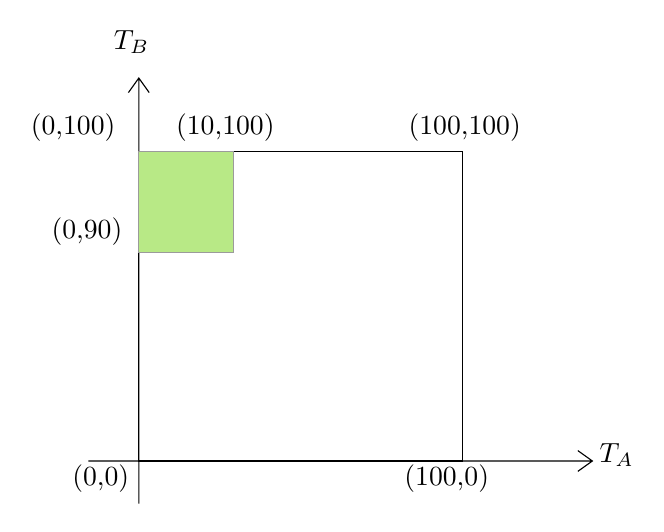
\begin{tikzpicture}[x=0.75pt,y=0.75pt,yscale=-1,xscale=1]
%uncomment if require: \path (0,300); %set diagram left start at 0, and has height of 300

%Shape: Axis 2D [id:dp6343355519100857] 
\draw  (50,260.5) -- (292.8,260.5)(74.28,76) -- (74.28,281) (285.8,255.5) -- (292.8,260.5) -- (285.8,265.5) (69.28,83) -- (74.28,76) -- (79.28,83)  ;
%Shape: Rectangle [id:dp3216026959076823] 
\draw   (74.28,111.5) -- (230.28,111.5) -- (230.28,260.5) -- (74.28,260.5) -- cycle ;
%Shape: Rectangle [id:dp2814567082553894] 
\draw  [color={rgb, 255:red, 155; green, 155; blue, 155 }  ,draw opacity=1 ][fill={rgb, 255:red, 184; green, 233; blue, 134 }  ,fill opacity=1 ] (74.28,111.5) -- (120,111.5) -- (120,160) -- (74.28,160) -- cycle ;

% Text Node
\draw (41,261) node [anchor=north west][inner sep=0.75pt]   [align=left] {(0,0)};
% Text Node
\draw (201,261) node [anchor=north west][inner sep=0.75pt]   [align=left] {(100,0)};
% Text Node
\draw (203,92) node [anchor=north west][inner sep=0.75pt]   [align=left] {(100,100)};
% Text Node
\draw (21,92) node [anchor=north west][inner sep=0.75pt]   [align=left] {(0,100)};
% Text Node
\draw (295,251) node [anchor=north west][inner sep=0.75pt]   [align=left] {$T_A$};
% Text Node
\draw (61,52) node [anchor=north west][inner sep=0.75pt]   [align=left] {$T_B$};
% Text Node
\draw (31,142) node [anchor=north west][inner sep=0.75pt]   [align=left] {(0,90)};
% Text Node
\draw (91,92) node [anchor=north west][inner sep=0.75pt]   [align=left] {(10,100)};


\end{tikzpicture} \\

Since $T_A$ and $T_B$ are uniformly distributed, we can compute the probability as follows: \\ 

P = \dfrac{Desired Area}{Total Area} = \dfrac{10 . 10}{100 . 100} = \dfrac{1}{100} \newpage

\section*{c)} \\ 
The event is E = \{$T_A - T_B$ \leq 20\}. \\ \\

\noindent Since $T_A$ and $T_B$ are uniformly distributed, the probability can be found as follows: \\

\tikzset{every picture/.style={line width=0.75pt}} %set default line width to 0.75pt        

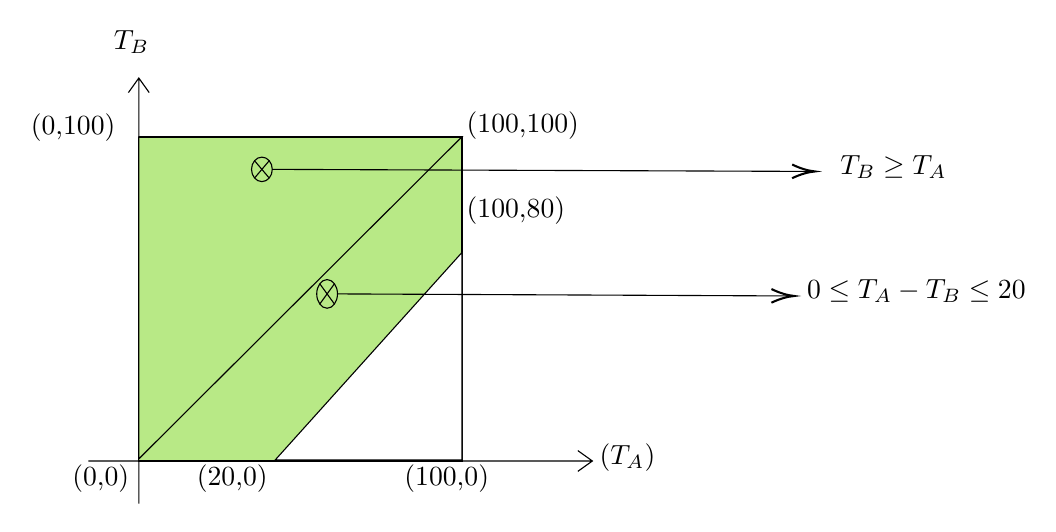
\begin{tikzpicture}[x=0.75pt,y=0.75pt,yscale=-1,xscale=1]
%uncomment if require: \path (0,300); %set diagram left start at 0, and has height of 300

%Shape: Axis 2D [id:dp6343355519100857] 
\draw  (50,260.5) -- (292.8,260.5)(74.28,76) -- (74.28,281) (285.8,255.5) -- (292.8,260.5) -- (285.8,265.5) (69.28,83) -- (74.28,76) -- (79.28,83)  ;
%Shape: Square [id:dp6167660680382179] 
\draw  [color={rgb, 255:red, 0; green, 0; blue, 0 }  ,draw opacity=1 ][fill={rgb, 255:red, 184; green, 233; blue, 134 }  ,fill opacity=1 ] (74.28,104.78) -- (230,104.78) -- (230,260.5) -- (74.28,260.5) -- cycle ;
%Shape: Right Triangle [id:dp5835632232925498] 
\draw  [fill={rgb, 255:red, 255; green, 255; blue, 255 }  ,fill opacity=1 ] (140,260) -- (230,160) -- (230,260) -- cycle ;
%Shape: Right Triangle [id:dp9870953547850405] 
\draw   (230,104.28) -- (74.28,259.5) -- (74.28,104.28) -- cycle ;
%Shape: Boxed Line [id:dp3089802335683467] 
\draw    (170,180) -- (388,180.99) ;
\draw [shift={(390,181)}, rotate = 180.26] [color={rgb, 255:red, 0; green, 0; blue, 0 }  ][line width=0.75]    (10.93,-3.29) .. controls (6.95,-1.4) and (3.31,-0.3) .. (0,0) .. controls (3.31,0.3) and (6.95,1.4) .. (10.93,3.29)   ;
%Shape: Boxed Line [id:dp5908192331926827] 
\draw    (138.58,120) -- (163.15,120.09) -- (237.66,120.38) -- (398,120.99) ;
\draw [shift={(400,121)}, rotate = 180.22] [color={rgb, 255:red, 0; green, 0; blue, 0 }  ][line width=0.75]    (10.93,-3.29) .. controls (6.95,-1.4) and (3.31,-0.3) .. (0,0) .. controls (3.31,0.3) and (6.95,1.4) .. (10.93,3.29)   ;
%Flowchart: Summing Junction [id:dp7766826126849855] 
\draw   (128.58,120) .. controls (128.58,116.74) and (130.82,114.1) .. (133.58,114.1) .. controls (136.34,114.1) and (138.58,116.74) .. (138.58,120) .. controls (138.58,123.26) and (136.34,125.9) .. (133.58,125.9) .. controls (130.82,125.9) and (128.58,123.26) .. (128.58,120) -- cycle ; \draw   (130.04,115.83) -- (137.11,124.17) ; \draw   (137.11,115.83) -- (130.04,124.17) ;
%Flowchart: Summing Junction [id:dp5985473951812927] 
\draw   (160,180) .. controls (160,176.19) and (162.24,173.1) .. (165,173.1) .. controls (167.76,173.1) and (170,176.19) .. (170,180) .. controls (170,183.81) and (167.76,186.9) .. (165,186.9) .. controls (162.24,186.9) and (160,183.81) .. (160,180) -- cycle ; \draw   (161.46,175.12) -- (168.54,184.88) ; \draw   (168.54,175.12) -- (161.46,184.88) ;

% Text Node
\draw (41,261) node [anchor=north west][inner sep=0.75pt]   [align=left] {(0,0)};
% Text Node
\draw (201,261) node [anchor=north west][inner sep=0.75pt]   [align=left] {(100,0)};
% Text Node
\draw (231,91) node [anchor=north west][inner sep=0.75pt]   [align=left] {(100,100)};
% Text Node
\draw (21,92) node [anchor=north west][inner sep=0.75pt]   [align=left] {(0,100)};
% Text Node
\draw (295,251) node [anchor=north west][inner sep=0.75pt]   [align=left] {$(T_A)$};
% Text Node
\draw (61,52) node [anchor=north west][inner sep=0.75pt]   [align=left] {$T_B$};
% Text Node
\draw (101,261) node [anchor=north west][inner sep=0.75pt]   [align=left] {(20,0)};
% Text Node
\draw (231,132) node [anchor=north west][inner sep=0.75pt]   [align=left] {(100,80)};
% Text Node
\draw (411,112) node [anchor=north west][inner sep=0.75pt]   [align=left] {$T_B \geq T_A$};
% Text Node
\draw (395,172) node [anchor=north west][inner sep=0.75pt]   [align=left] {$0 \leq T_A - T_B \leq 20$};


\end{tikzpicture}
\newline 
P(E) = \dfrac{DesiredArea}{TotalArea} = \dfrac{6800}{1000} = \dfrac{68}{100}

$\newline \newline \\ \\$
\section*{d)}
They fail if $|T_A - T_B| > 30$ . \\ \\
So, they pass the test  $|T_A - T_B| \leq 30$, which also means they pass if $-30 \leq T_A - T_b \leq 30$.



\tikzset{every picture/.style={line width=0.75pt}} %set default line width to 0.75pt        

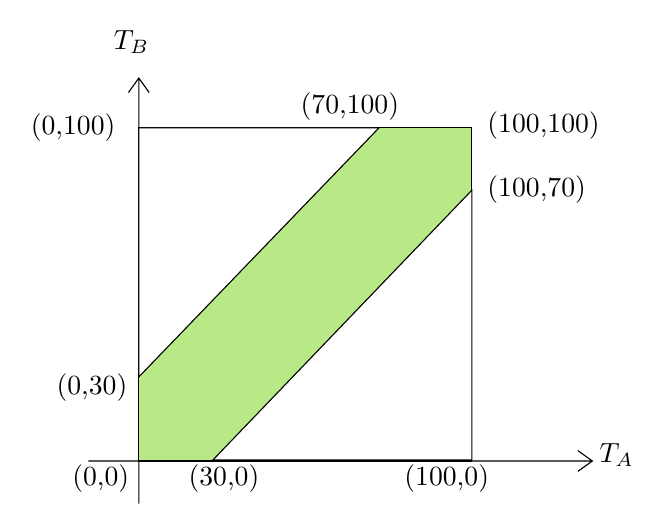
\begin{tikzpicture}[x=0.75pt,y=0.75pt,yscale=-1,xscale=1]
%uncomment if require: \path (0,300); %set diagram left start at 0, and has height of 300

%Shape: Axis 2D [id:dp6343355519100857] 
\draw  (50,260.5) -- (292.8,260.5)(74.28,76) -- (74.28,281) (285.8,255.5) -- (292.8,260.5) -- (285.8,265.5) (69.28,83) -- (74.28,76) -- (79.28,83)  ;
%Shape: Square [id:dp6577379627539568] 
\draw  [fill={rgb, 255:red, 184; green, 233; blue, 134 }  ,fill opacity=1 ] (74.28,100) -- (234.78,100) -- (234.78,260.5) -- (74.28,260.5) -- cycle ;
%Shape: Right Triangle [id:dp4248600749820899] 
\draw  [fill={rgb, 255:red, 255; green, 255; blue, 255 }  ,fill opacity=1 ] (190,100) -- (74.28,220) -- (74.28,100) -- cycle ;
%Shape: Right Triangle [id:dp5313600397781888] 
\draw  [fill={rgb, 255:red, 255; green, 255; blue, 255 }  ,fill opacity=1 ] (110,260) -- (234.78,130) -- (234.78,260) -- cycle ;

% Text Node
\draw (41,261) node [anchor=north west][inner sep=0.75pt]   [align=left] {(0,0)};
% Text Node
\draw (201,261) node [anchor=north west][inner sep=0.75pt]   [align=left] {(100,0)};
% Text Node
\draw (241,91) node [anchor=north west][inner sep=0.75pt]   [align=left] {(100,100)};
% Text Node
\draw (21,92) node [anchor=north west][inner sep=0.75pt]   [align=left] {(0,100)};
% Text Node
\draw (295,251) node [anchor=north west][inner sep=0.75pt]   [align=left] {$T_A$};
% Text Node
\draw (61,52) node [anchor=north west][inner sep=0.75pt]   [align=left] {$T_B$};
% Text Node
\draw (80,225) node   [align=left] {\begin{minipage}[lt]{68pt}\setlength\topsep{0pt}
(0,30)
\end{minipage}};
% Text Node
\draw (151,82) node [anchor=north west][inner sep=0.75pt]   [align=left] {(70,100)};
% Text Node
\draw (241,122) node [anchor=north west][inner sep=0.75pt]   [align=left] {(100,70)};
% Text Node
\draw (97,261) node [anchor=north west][inner sep=0.75pt]   [align=left] {(30,0)};


\end{tikzpicture}

Since $T_A$ and $T_B$ are independent, the probability can be found as follows: \\

P(pass) = \dfrac{DesiredArea}{TotalArea} = \dfrac{5100}{10000} = \dfrac{51}{100}

\newpage
\section*{Answer 3}

\section*{a)} \\
Note that cdf of an exponential random variable X with $\lambda$ is.
F(t) = P(X \leq t) = 1 - $e^{-\lambda t}$ \\
So, complement of it is 
P(X $>$ t) = $e^{-\lambda t}$.\\ \\
\noindent Now, we will examine T = min$(X_1,X_2,.....,X_n)$ more closely. \\ 

\noindent If we want P(T $>$ t) for some t $>$ 0, we just want \\ 

\noindent P(T $>$ t) = P(min$(X_1,X_2,.....,X_N) > $ t) = P($X_1 > t$, $X_2 > t$,....,$X_n > t$) \\ \\ = P($X_1 > $ t) .   P($X_2 > $ t) . .......  .P($X_n > $ t)  \\ \\
= $e^{-\lambda_1 t}$ . $e^{-\lambda_2 t}$. ....... . $e^{-\lambda_n t}$ \\ \\
= $e^{-(\lambda_1 + \lambda_2 + ..... + \lambda_n)t}$ \\ \\ \\ 

\noindent So, we found P(T $>$ t) =  $e^{-(\lambda_1 + \lambda_2 + ..... + \lambda_n)t}$. And now we can find $F_T(t)$, cdf of T. \\ \\

\noindent $F_T(t)$ = P (T \leq t) = 1 - P(T > t) = 1 - $e^{-(\lambda_1 + \lambda_2 + ..... + \lambda_n)t}$ \\ \\

\noindent As you can see above, T itself is exponential with $\lambda = \lambda_1 + \lambda_2 + ..... \lambda_n$ and cdf $F_T(t)$ \\

\begin{center}
    $F_T(t)$ = 1 - $e^{-(\lambda_1 + \lambda_2 + ..... + \lambda_n)t}$
\end{center}
\newpage


\section*{b)} \\
\indent Let $X_1 , X_2, ... X_n$ be independent exponential random variables with $\lambda_i$ for i = 1,2,....n,  and  \\ T = min$(X_1,X_2,.....,X_n)$. \\ \\

\noindent Now, let's investigate complement of cdf of T. \\\\
\noindent P(T $>$ t) = P(min$(X_1,X_2,.....,X_N) > $ t) = P($X_1 > t$, $X_2 > t$,....,$X_n > t$) \\ \\ = P($X_1 > $ t) .   P($X_2 > $ t) . .......  P($X_n > $ t)  \\ \\
= $e^{-\lambda_1 t}$ . $e^{-\lambda_2 t}$. ....... . $e^{-\lambda_n t}$ \\ \\
= $e^{-(\lambda_1 + \lambda_2 + ..... + \lambda_n)t}$ \\ \\ 

\noindent So, cdf of T, $F_T(t) = $ 1 - $e^{-(\lambda_1 + \lambda_2 + ..... + \lambda_n)t}$ \\ \\

\noindent This shows that \textbf{T itself is also an exponential random variable.} \\
Hence, we get the below fact: \\ \\
\textbf{Fact:} Let $X_1 , X_2, ... X_n$ be independent exponential random variables with $\lambda_i$ for i = 1,2,....n. Then, T = min$(X_1,X_2,.....,X_n)$ is also an exponential random variable with $\lambda = 
\lambda_1 + \lambda_2 + ........ \lambda_n $ . \\ \\

\noindent The question is asking for E(T = min$(C_1,C_2,.....,C_{10})$) . \\ \\

\noindent Since E($C_n$) = $ \dfrac{10}{n}$ for $n = 1,2, .... 10$, we get $\lambda_n$ = \dfrac{n}{10} for $ n = 1,2,...,10$ \\ \\

\noindent Then, $\lambda_T$ = $\lambda_1 + \lambda_2 + ...... + \lambda_{10}$ = \dfrac{1+2+3+4+5+6+7+8+9+10}{10} = \dfrac{55}{10} \\ \\

\noindent Therefore, the expected time before one of the computer fails, E(T) \\ \\

\begin{center}
    E(T) =  $\dfrac{1}{\lambda_T} = \dfrac{10}{55} = \dfrac{2}{11}$
\end{center}




\newpage
\section*{Answer 4}
\section*{a)}

The number X of undergraduate students has \textbf{binomial distribution} with \\ \\

\indent n = 100 \\
\indent p = 0.74 \\
\indent $\mu$ = np = 74 \\
\indent $\sigma$ = \sqrt{np(1-p)} = 4.3863 \\ \\

\noindent Applying the Central Limit Theorem with the continuity correction, \\ \\

P(X \geq \dfrac{70}{100} . 100) = P(X \geq 70) = 1 - P(X < 70) \\ \\
\indent = 1 - P(X < 69.5) = 1 - P(\dfrac{X  - 74}{4.3863} \leq \dfrac{69.5 - 74}{4.3863}) \\ \\
\indent = 1 - $\phi(-1.0259)$ = 1 - $\phi(-1.03)$ = 1 - 0.1515 = \textbf{0.8485}. \\ \\

\noindent \textbf{Answer} = 0.8485 \\

\section*{b)}

The number X of participants pursuing a doctoral degree has \textbf{binomial distribution} with \\ \\

\indent n = 100 \\
\indent p = 0.10 \\
\indent $\mu$ = np = 10 \\
\indent $\sigma$ = \sqrt{np(1-p)} = 3 \\ \\

\noindent Applying the Central Limit Theorem with the continuity correction, \\ \\

 P(X \leq \dfrac{5}{100}. 100) = P(X \leq 5) = P(X \leq 5.5) = \\ \\
\indent = P(\dfrac{x-10}{3} < \dfrac{5.5 - 10}{3}) = $\phi(-1.5)$ = \textbf{0.0668} \\ \\

\noindent \textbf{Answer} = 0.0668 \\ \\

\noindent \textbf{(Values of standart normal distribution cdf, $\phi$, was taken from TABLE A4 in textbook.) } 



\end{document}
